%++++++++++++++++++++++++++++++++++++++++
% Don't modify this section unless you know what you're doing!
\documentclass[letterpaper,12pt]{article}
\usepackage{tabularx} % extra features for tabular environment
\usepackage{amsmath}  % improve math presentation
\usepackage{graphicx} % takes care of graphic including machinery
\renewcommand{\thefigure}{\arabic{section}.\arabic{figure}}
\usepackage{float}
\usepackage{subcaption}
\usepackage{algorithm}
\usepackage{algpseudocode}
\usepackage[margin=1in,letterpaper]{geometry} % decreases margins
\usepackage{cite} % takes care of citations
\setlength {\marginparwidth }{2cm} % needed for todonotes to work properly
\usepackage{todonotes}
\usepackage[toc,acronym, nonumberlist, style=super,nogroupskip]{glossaries} % acronyms use \gls \glspl \Gls \Glspl 
\usepackage[final]{hyperref} % adds hyper links inside the generated pdf file
\hypersetup{
	colorlinks=true,       % false: boxed links; true: colored links
	linkcolor=blue,        % color of internal links
	citecolor=blue,        % color of links to bibliography
	filecolor=magenta,     % color of file links
	urlcolor=blue         
}
\usepackage{cleveref} % takes care cross-references

\newacronym{ASC}{ASC}{Autonomous Surface Craft}
\newacronym{SFM}{SFM}{Structure From Motion}
\newacronym{ACFR}{ACFR}{Australian Center for Field Robotics}
\newacronym{PCL}{PCL}{Point Cloud Library}
\newacronym{FPFH}{FPFH}{Fast Point Feature Histograms}
\newacronym{RANSAC}{RANSAC}{RANdom SAmple Consensus}
\newacronym{CIRS}{CIRS}{Centre d'Investigació en Robòtica Submarina}
\newacronym{ROS}{ROS}{Robot Operating System}
\newacronym{IMR}{IMR}{Inspection Maintenance and Repair}
\newacronym{FEKFSLAM}{EKFFSLAM}{Feature Based EKF SLAM}
\newacronym{PEKFSLAM}{PEKFSLAM}{Pose based EKF SLAM}
\newacronym{FMBL}{FMBL}{Feature Map Based Localization}
\newacronym{MBL}{MBL}{Map Based Localization}
\newacronym{MRU}{MRU}{Motion Reference Unit}
\newacronym{HS}{HS}{Hough Space}
\newacronym{FIFO}{DIDO}{First Input First Output}
\newacronym{IDP}{IDP}{Inverse-Depth Parameterization}
\newacronym{SBUSLAM}{SBUSLAM}{Single Beacon Underwater Simultaneous Localization And Mapping}
\newacronym{SBBOSLAM}{SBBOSLAM}{Single Beacon Bearing Only Simultaneous Localization And Mapping}
\newacronym{pdf}{pdf}{probability density function}
\newacronym{cdf}{cdf}{cumulative density function}
\newacronym{ICNN}{ICNN}{Individual Compatibility Nearest Neighbour}
\newacronym{JCBB}{JCBB}{Joint Compatibility Branch and Bound}
\newacronym{ECI}{ECI}{Earth Centered Earth Fixed}
\newacronym{ECEF}{ECEF}{Earth Centered Inertial}
\newacronym{NED}{NED}{North East Down}
\newacronym{WGS84}{WGS84}{World Geodetic system 1984}
\newacronym{RPY}{RPY}{Roll-Pitch-Yaw}
\newacronym{PMM}{PMM}{Planar Motion Mechanism}
\newacronym{PMB}{PMB}{Parallel Midbody Hull}
\newacronym{DR}{DR}{Dead Reckoning}
\newacronym{CFD}{CFD}{Computational Fluid Dynamics}
\newacronym{IMU}{IMU}{Inertial Measurement Unit}
\newacronym{INS}{INS}{Inertial Navigation System}
\newacronym{USBL}{USBL}{Ultra Short Base Line}
\newacronym{SBL}{SBL}{Short Base Line}
\newacronym{LBL}{LBL}{Long Base Line}
\newacronym{GIB}{GIB}{GPS Equipped Buoys}
\newacronym{ILBL}{IBL}{Inverted Long Base Line}
\newacronym{VLBL}{VLBL}{Virtual Long Base Line}
\newacronym{DGPS}{DGPS}{Differential Gobal Position System}
\newacronym{GPS}{GPS}{Gobal Position System}
\newacronym{AHRS}{AHRS}{Attitude and Heading Reference System}
\newacronym{DVL}{DVL}{Doppler Velocity Log}
\newacronym{EKF}{EKF}{Extended Kalman Filter}
\newacronym{EIF}{EIF}{Extended Information Filter}
\newacronym{KF}{KF}{Kalman Filter}
\newacronym{UKF}{UKF}{Unscented Kalman Filter}
\newacronym{IF}{IF}{Information Filter}
\newacronym{BF}{BF}{Bayes Filter}
\newacronym{HF}{HF}{Histogram Filter}
\newacronym{GRV}{GRV}{Gaussian Random Vector}
\newacronym{RV}{RV}{Random Vector}
\newacronym{UAV}{UAV}{Unmanned Aerial Vehicle}
\newacronym{AUV}{AUV}{Autonomous Underwater Vehicle}
\newacronym{UUV}{UUV}{Unmanned Underwater Vehicle}
\newacronym{ROV}{ROV}{Remotely Operated Vehicle}
\newacronym{SSS}{SSS}{Side Scan Sonar}
\newacronym{SAS}{SAS}{Synthetic Apperture Sonar}
\newacronym{MBES}{MBES}{Multi Beam Echo Sounder}
\newacronym{SBES}{SBES}{Singe Beam Echo Sounder}
\newacronym{FLS}{FLS}{Forward Looking Sonar}
\newacronym{MSIS}{MSIS}{Mechanical Scaning Imaging Sonar}
\newacronym{SBN}{SBN}{Single Beacon Navigation}
\newacronym{TBN}{TBN}{Terrain Based Navigation}
\newacronym{OGM}{OGM}{Occupancy Grid Mapping}
\newacronym{OM}{OM}{Occupancy Mapping}
\newacronym{SLAM}{SLAM}{Simultaneous Localization and Mapping}
\newacronym{DOF}{DOF}{Degree Of Freedom}
\newacronym{PDF}{PDF}{Probability Density Function}
\newacronym{SVD}{SVD}{Single Value Decomposition}
\newacronym{ICP}{ICP}{Iterative Closest Point}
\newacronym{PF}{PF}{Particle Filter}
\newacronym{MCL}{MCL}{Montecarlo Localization}
\newacronym{GL}{GL}{Grid Localization}
\newacronym{ML}{ML}{Markovian Localization}
\newacronym{MSSP}{MSSP}{Mechanical Scanning Sonar Profiler}
\newacronym{HMM}{HMM}{Hidden Markov Model}
\newacronym{MP}{MP}{Markov Process}
\newacronym{BN}{BN}{Bayesian Network}
\newacronym{DBN}{DBN}{Dynamic Bayesian Network}
\newacronym{BR}{BR}{Bayes Rule}
\newacronym{PNP}{PNP}{Perspective-n-Point}
\newacronym{LGS}{LGS}{Linear Gaussian System}
\newacronym{CFG}{CFG}{computed Fluid Dynamics}
\newacronym{ESS}{ESS}{Effective Sample Size}
\newacronym{ULS-RO}{ULS-RO}{Unconstrained Least Squares Range-Only Localization}
\newacronym{DTM}{DTM}{Digital Terrain Model}
\newacronym{LS}{LS}{Least Squares}
\newacronym{ULS}{ULS}{Unconstrained Least Squares}
\newacronym{WLS}{WLS}{Weighted Least Squares}
\newacronym{TDOA}{TDOA}{Time Difference OF Arrivals}
\newacronym{TOF}{TOF}{Time Of Fly}
\newacronym{LTI}{LTI}{Linear Time Invariant}
\newacronym{LTV}{LTV}{Linear Time Variant}
\newacronym{ORC}{ORC}{Observability Rank Condition}
\newacronym{LWO}{LWO}{Locally Weakly Observable}
\newacronym{SPL}{SPL}{Sound Pressure Level}
\newacronym{LRF}{LRF}{Laser Range Finder}
\newacronym{SPW}{SPW}{Sound Power}
\newacronym{SP}{SP}{Sound Pressure}
\newacronym{SI}{SI}{Sound Intensity}
\newacronym{SE}{SE}{Sound Energy}
\newacronym{SIL}{SIL}{Sound Intensity Level}
\newacronym{CGW}{CGW}{Continuous Gated Wave}
\newacronym{FIR}{FIR}{Finit Impulse Response}
\newacronym{SNR}{SNR}{Signal-to-noise Ratio}
\newacronym{LFM}{LFM}{Linear Frequency Modulated}
\newacronym{COTS}{COTS}{commercial of the shelf}
\newacronym{FFT}{FFT}{Fast Fourier Transform}
\newacronym{SVP}{SVP}{Sound Velocity Profile}
\newacronym{MSV}{MSV}{Mean Sound Velocity}
\newacronym{ISSS}{ISSS}{Interferometic Side Scan Sonar}
\newacronym{SBSSS}{SBSSS}{Swath Bathymetry Side Scan Sonar}
\newacronym{MIS}{MIS}{Multibeam Imaging Sonars}
\newacronym{BMIS}{BMIS}{Beam forming Multibeam Imaging Sonar}
\newacronym{IMIS}{IMIS}{Inteferometric Multibeam Imaging Sonar}
\newacronym{LMIS}{LMIS}{Lenses based Multibeam Imaging Sonar}
\newacronym{DIDSON}{DIDSON}{Dual frequency IDentification SONar}
\newacronym{SONAR}{SONAR}{SOund NAvigation and Ranging}
\newacronym{DPCA}{DPCA}{Displaced Phase Center Antenna }
\newacronym{SAUC-E}{SAUC-E}{Student Autonomous Underwater Challenge-Europe} 

%++++++++++++++++++++++++++++++++++++++++


\begin{document}

\title{Differential Drive Mobile Robot Simulation and Dead Reckoning}
\author{Loc Pham,  and Mohamed Khaled}
\date{\today}
\maketitle

\begin{abstract}
\textcolor{black}{This lab report presents the simulation of a differential drive mobile robot, focusing on motion modeling and the implementation of dead reckoning techniques. The mobile robot operates within two frames: the N-frame, the world frame, and the robot body frame, the B-frame. The primary objective of this study was to program the robot simulation to execute two distinct trajectory paths, namely a circular trajectory and an 8-shaped trajectory. To achieve these predefined motion paths, the robot's motion is simulated by specifying a desired velocity and radius for the circular path. This investigation underscores the critical role of motion modeling and the application of dead reckoning in guiding mobile robots through complex trajectories}
\end{abstract}

% \section{Methodology}
% \textcolor{blue}{Briefly describe what was done in the \emph{Pre-Lab}, the \emph{Lab session} and the \emph{Post-Lab}}
% This lab involved 3 steps:
% \begin{enumerate}
%     \item \textbf{Pre-Lab:} The Pre-Lab consisted in...
   
%     \item \textbf{Lab-Session}: The Lab session involved ...
%     \item \textbf{Post-Lab}: After the lab session we had to ...
% \end{enumerate}


\section{Introduction}
\textcolor{black}{The objective of this lab was the understanding and simulation of the behavior of a differential drive mobile robot, with a focus on simulating their motion models and applying the concept of dead reckoning. For more organized and easy implementation,  a GitHub repository had been used; which contained blueprint classes designed for robot simulation. Moreover, the Pose3D class had been implemented to represent a three-dimensional pose. This class featured two critical methods: "oplus" and "ominus." The "oplus" method enabled us to efficiently compound points in different frames, thereby facilitating forward compounding, such as AxB $\oplus$  BxC = AxC. Conversely, the "ominus" method allowed for the reverse compounding of points, exemplified in the form of CxA =  $ \ominus $ AxC}.\\
\\This reports is organized as follows: \Cref{sec:Simulation} describes how to simulate the robot by implementing the \emph{DifferentialDriveSimulatedRobot} class inheriting from the \emph{SimulatedRobot} base class. This section also explains how to use the class to simulate the trajectories requested in the lab. \Cref{sec:Dead-Reckoning} details the dead reckoning localization method of a differential drive mobile robot. The technique is implemented in the \emph{DR\_3DOFDifferentialDrive} class as a child class of the \emph{Localization} class providing an implementation for their virtual methods. Finally, the \cref{sec:Issues} is devoted to the description of the problems founds during the lab.

\section{Simulation}
\label{sec:Simulation}
In this lab report, a detailed methodology is illustrated to simulate a differential drive robot. The primary objective was to create a simulated model capable of emulating the motion and sensor outputs of the robot. To achieve this, we utilized the DifferentialDriveSimulatedRobot class, which updates the robot’s current position using \textit{fs()} class method. Moreover, all the mentioned classes have been tested for our simulated robot, and the results have been analyzed and explained to illustrate the differences between the desired trajectory and the robot trajectory. This evaluation verifies the accuracy and reliability of the simulation model using only a P controller. The figure \ref{fig:00} below shows the design of a simulation, which contains simulation system (robot modeling, sensors modeling and so on) and navigation system.
\begin{figure}[H]
\centering
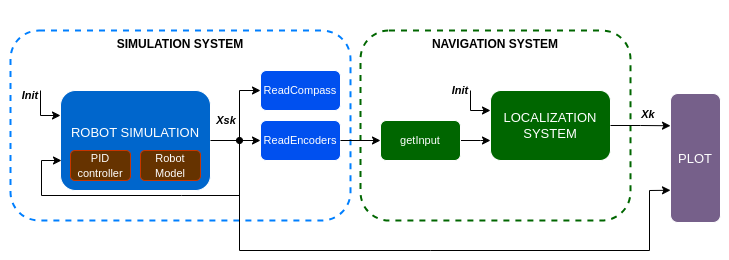
\includegraphics[width=16cm]{Figures/system_design.png}
\caption{The simulation design}
\label{fig:00}
\end{figure}

\subsection{ Robot Simulation}
\label{sec:robotSimulation}
To begin with the simulation of robot motion, a custom function, \textit{fs()}, was developed. This function is designed to calculate the current state, ${X_{sk}}$, of the robot based on its preceding state, ${X_{sk-1}}$, and the desired input, ${U_{k}}$. The state ${X_{sk-1}}$ is represented as a 6x1 matrix, with the initial three elements corresponding to the robot's pose, and the subsequent three elements representing the robot's velocity.
To control the simulated velocity towards the desired input, a diagonal matrix, \textit{K}, was employed as a simple P controller. Furthermore, the acceleration term, ${w_{sk}}$, was incorporated into the simulation to introduce the real robot noise in the robot's velocity during its motion; for more realism of the simulated robot motion. \cite{Lectures}, \cite{Book} and \cite{SoftwareDesign} 

\begin{equation}
    \label{eq:prev_pose}
\begin{aligned}
    X_{sk-1} =
    \begin{bmatrix}
   \eta_{sk-1}\\ \nu_{sk-1} 
   \\ \end{bmatrix}
    \end{aligned}
\end{equation}
\begin{equation}
    \label{eq:current_pose}
\begin{aligned}
    X_{sk} =
    \begin{bmatrix}
   \eta_{sk-1} \oplus (\nu_{sk-1}\Delta t + \frac{1}{2} w_{sk} \Delta t^2 )\\  (\nu_{sk-1} + K(\nu_{d} - \nu_{sk-1}) + w_{sk} \Delta t\\ \end{bmatrix}
\end{aligned}
\end{equation}


\subsection{Simulation Test}
\label{sec:SimulationTest}
This section explains how to simulate the robot with circular and figure-8 trajectories. In this section, the requested trajectories, the explanation of the code, and the problems encountered have been illustrated as follows.

\begin{figure}[H]
    \centering
    \begin{subfigure}[b]{6.5cm}
        \centering
        \frame{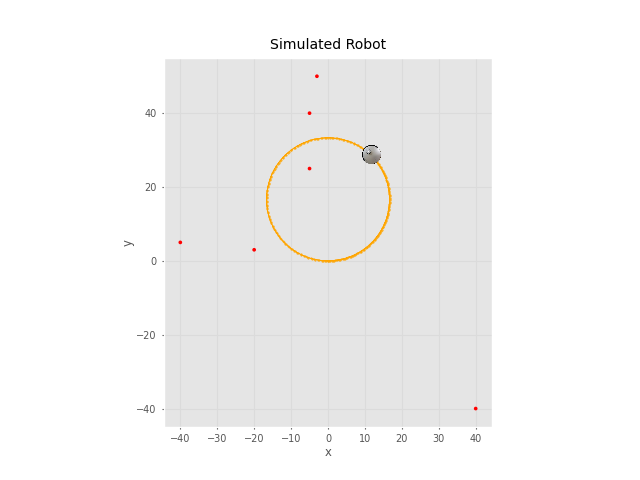
\includegraphics[width=6.0cm]{Figures/1.Simulation/o_trajectory_accNoise_0.0.png}}
        \captionsetup{justification=centering}
        \caption{No noise}
        \label{fig:kermit}
    \end{subfigure}
    % \hfill
    \begin{subfigure}[b]{6.5cm}
        \centering
        \frame{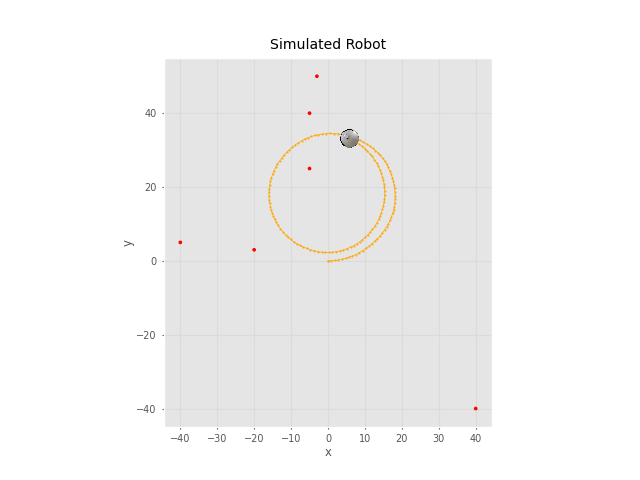
\includegraphics[width=6.0cm]{Figures/1.Simulation/o_trajectory_accNoise_0.5.png}}
        \captionsetup{justification=centering}
        \caption{Standard deviation: [1.0, 0.0, 0.17]}
        \label{fig:rana}
    \end{subfigure}
\caption{The position of simulated robot with circular trajectory}
\label{fig:map2_1}
\end{figure}

\begin{figure}[H]
    \centering
    \begin{subfigure}[b]{6.5cm}
        \centering
        \frame{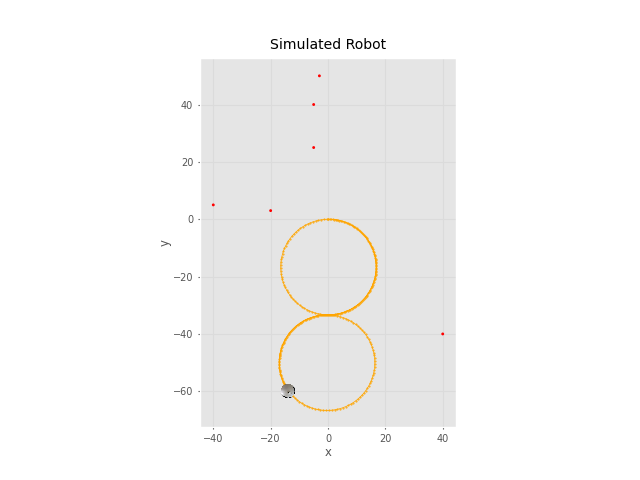
\includegraphics[width=6.0cm]{Figures/1.Simulation/8_trajectory_accNoise_0.0.png}}
        \captionsetup{justification=centering}
        \caption{No noise}
        \label{fig:kermit}
    \end{subfigure}
    % \hfill
    \begin{subfigure}[b]{6.5cm}
        \centering
        \frame{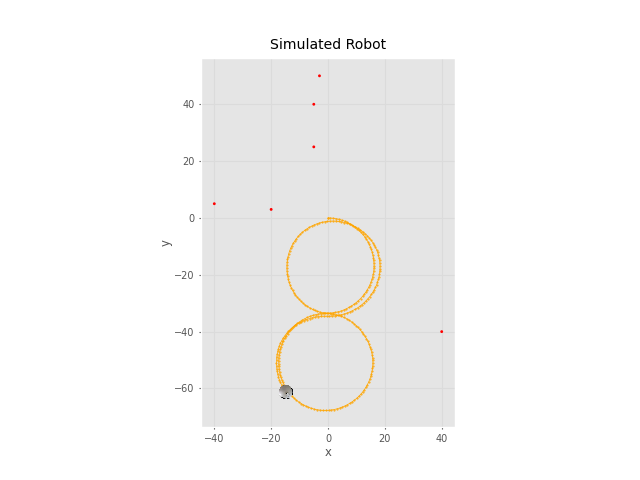
\includegraphics[width=6.0cm]{Figures/1.Simulation/8_trajectory_accNoise_0.5.png}}
        \captionsetup{justification=centering}
        \caption{Standard deviation: [1.0, 0.0, 0.17]}
        \label{fig:rana}
    \end{subfigure}
\caption{The position of simulated robot with 8-figure trajectory}
\label{fig:map2_2}
\end{figure}
\noindent
The results of simulation are represented in the figure \ref{fig:map2_1} and \ref{fig:map2_2} corresponding to two trajectories. Firstly, with the circular trajectory, we set the desired linear velocity and angular velocity of the robot represented in body-fixed frame is constants. The radius of circular trajectory can be calculated from these two configurations (radius $=$ linear velocity / angular velocity). Secondly, the 8-figure trajectory, we set up similarly to the circular trajectory, add a condition to change the sign for the angular velocity when robot has completed one circle, algorithm \ref{alg:1}. Beside, each figures contain two images, the first one is the result of a simulation with no noise while the second one is the result with the Zero-mean Gaussian model for acceleration noise (standard deviation is $[1.0, 0.0, 0.17]$). It is clear that robot did not get the desired trajectories with the acceleration noise. We will discuss it in the next paragraph.
\begin{algorithm}
\caption{8-figure Algorithm}\label{alg:1}
\begin{algorithmic}
\If{The X position of the robot moves from the positive region to the negative region
$[^N x_s(k-1) * ^N x_s(k) < 0.0$ and $^N x_s(k) \leq N x_s(k-1)$]}
\State angularVelocity = -angularVelocity
\\
\EndIf
\end{algorithmic}
\end{algorithm}

\noindent
In this paragraph, we discuss about the influences of acceleration noise on the simulation. In the simulation, we have the formula:
\begin{equation}
\label{equa:1}
\nu_{s_{k}} = \nu_{s_{k-1}} + u_{k-1} + w_{s_k} \Delta t
\end{equation}
with $u$ is considered as a control signal which controls the robot following the desired purposes, $\nu_{d}$ is the desired linear velocity and angular velocity of the robot represented in Body fixed Frame.
\begin{equation}
\label{equa:2}
u_{k-1} = K (\nu_{d} - \nu_{s_{k-1}})
\end{equation}
In the equation \ref{equa:2}, we use velocity controller (P controller), which makes the linear and angular velocity to track to desired ones. The simulated velocities and their desires are represented in the figure [\ref{fig:map2_3}, \ref{fig:map2_4}, \ref{fig:map2_5}] with situations: no noise and acceleration noise with Gaussian white noise model. However, because it is only the velocity controller, when adding acceleration noise to the simulation, the position of the robot will not reach the desired trajectory (circular and 8-figure trajectories).
\begin{figure}[H]
    \centering
    \begin{subfigure}[b]{8.cm}
        \centering
        \frame{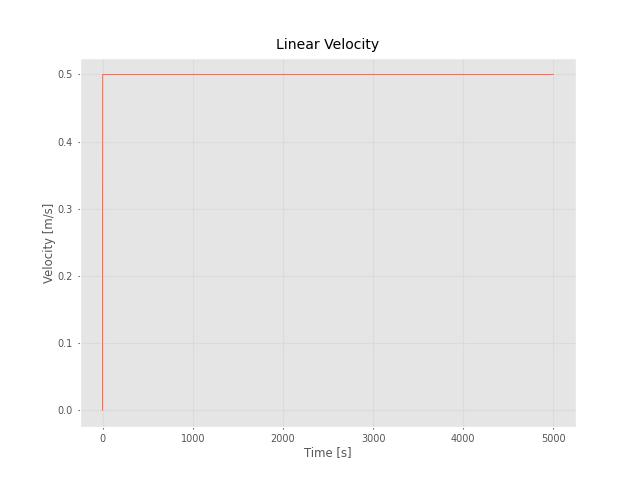
\includegraphics[width=7.00cm]{Figures/1.Simulation/linearVelocity_accNoise_0.0.png}}
        \captionsetup{justification=centering}
        \caption{Linear Velocity}
        \label{fig:kermit}
    \end{subfigure}
    % \hfill
    \begin{subfigure}[b]{8.cm}
        \centering
        \frame{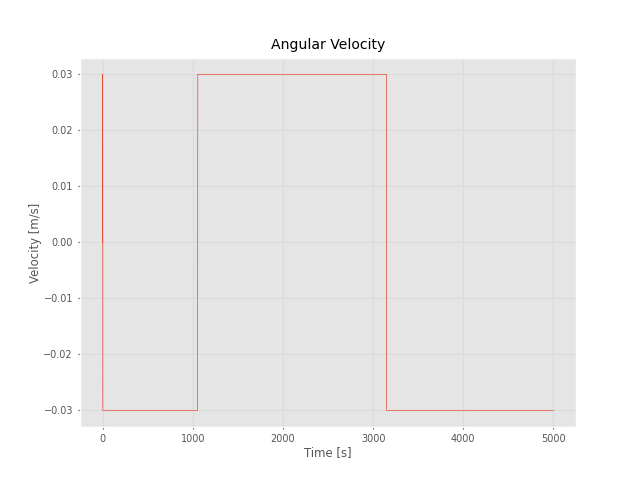
\includegraphics[width=7.0cm]{Figures/1.Simulation/angularVelocity_accNoise_0.0.png}}
        \captionsetup{justification=centering}
        \caption{Angular Velocity}
        \label{fig:rana}
    \end{subfigure}
\caption{The linear and angular velocity of the robot represented in body-fixed frame with no noise}
\label{fig:map2_3}
\end{figure}

\begin{figure}[H]
    \centering
    \begin{subfigure}[b]{8.cm}
        \centering
        \frame{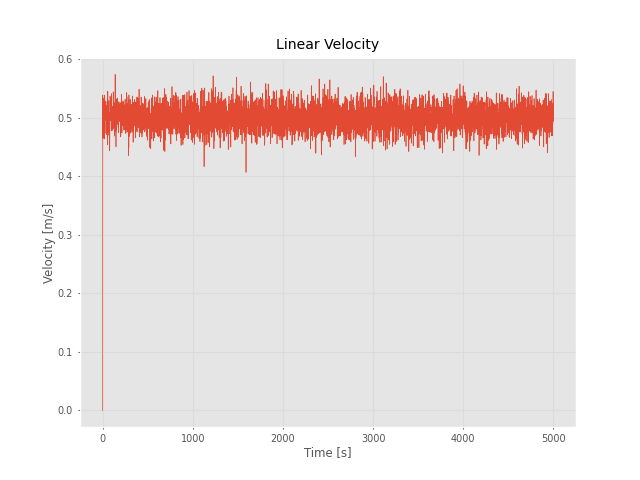
\includegraphics[width=7.00cm]{Figures/1.Simulation/linearVelocity_accNoise_0.2.png}}
        \captionsetup{justification=centering}
        \caption{Linear Velocity}
        \label{fig:kermit}
    \end{subfigure}
    % \hfill
    \begin{subfigure}[b]{8.cm}
        \centering
        \frame{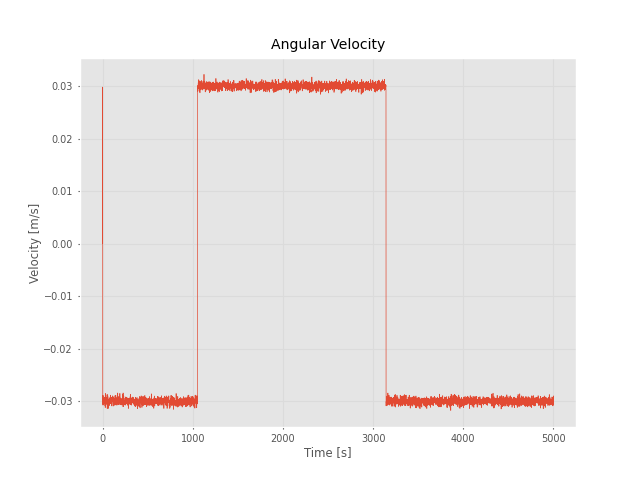
\includegraphics[width=7.0cm]{Figures/1.Simulation/angularVelocity_accNoise_0.005.png}}
        \captionsetup{justification=centering}
        \caption{Angular Velocity}
        \label{fig:rana}
    \end{subfigure}
\caption{The linear and angular velocity of the robot represented in body-fixed frame with the standard deviations are 0.2 and 0.005 respectively}
\label{fig:map2_4}
\end{figure}

\begin{figure}[H]
    \centering
    \begin{subfigure}[b]{8.cm}
        \centering
        \frame{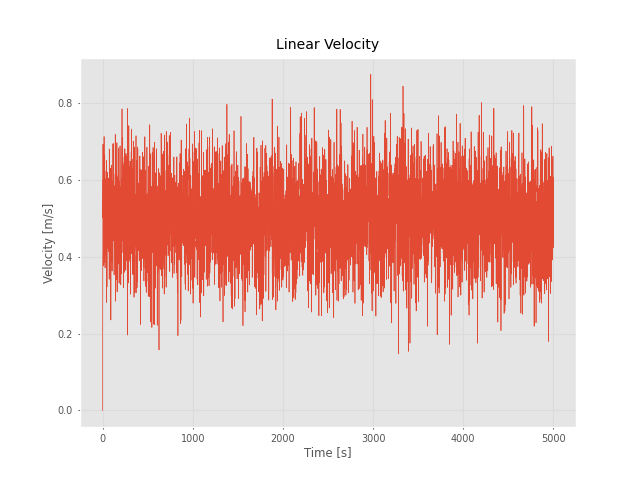
\includegraphics[width=7.00cm]{Figures/1.Simulation/linearVelocity_accNoise_1.0.png}}
        \captionsetup{justification=centering}
        \caption{Linear Velocity}
        \label{fig:kermit}
    \end{subfigure}
    % \hfill
    \begin{subfigure}[b]{8.cm}
        \centering
        \frame{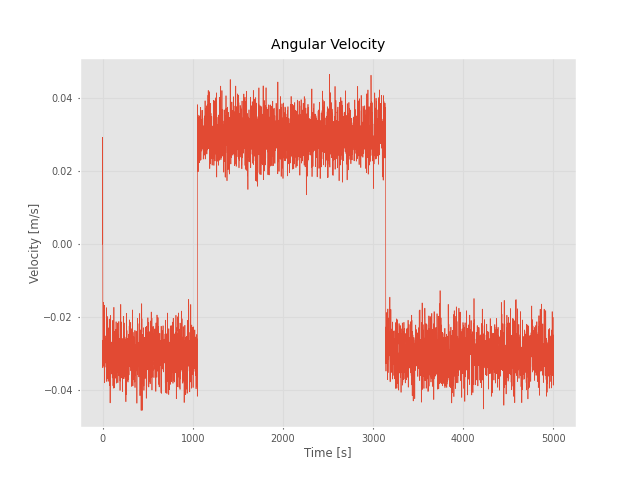
\includegraphics[width=7.0cm]{Figures/1.Simulation/angularVelocity_accNoise_0.05.png}}
        \captionsetup{justification=centering}
        \caption{Angular Velocity}
        \label{fig:rana}
    \end{subfigure}
\caption{The linear and angular velocity of the robot represented in body-fixed frame with the standard deviations are 1.0 and 0.05 respectively}
\label{fig:map2_5}
\end{figure}

\section{Dead-Reckoning}
\label{sec:Dead-Reckoning}
\setcounter{figure}{0}  
In navigation, dead reckoning is the process of calculating the current position of a moving object by using a previously determined position, or fix, and incorporating estimates of speed, heading (or direction or course), and elapsed time. In this project, the current position of the robot is computed from the previous position and travel distance of two wheels from encoder measurement. The figure \ref{fig:map3_1} shows the results of localization system compared to simulation position. It is clear that with no noise in the encoder output, the error between localization and simulation position is very small. Meanwhile, the figure \ref{fig:map3_2} illustrates the dead reckoning problem when adding Gaussian white noise with standard deviation is 22 to encoder output. Obviously, there is a big error between the position from the localization system and the simulation. 
\begin{figure}[H]
    \centering
    \begin{subfigure}[b]{8.cm}
        \centering
        \frame{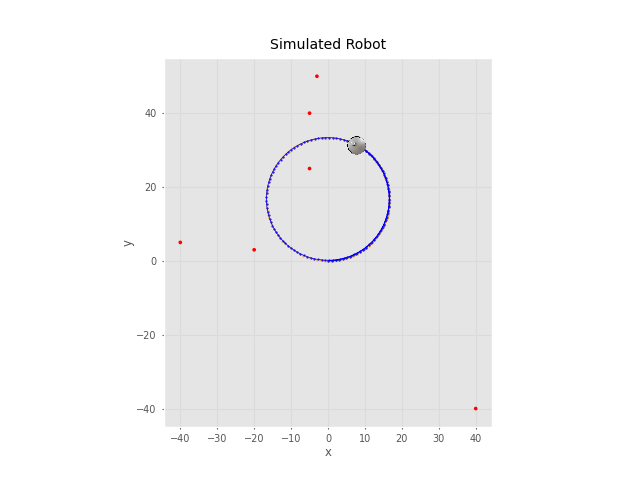
\includegraphics[width=7.00cm]{Figures/2.DeadReckoning/o_DR_noNoiseRecoder_noiseAcc.png}}
        \captionsetup{justification=centering}
        \caption{Circular trajectory}
        \label{fig:kermit}
    \end{subfigure}
    % \hfill
    \begin{subfigure}[b]{8.cm}
        \centering
        \frame{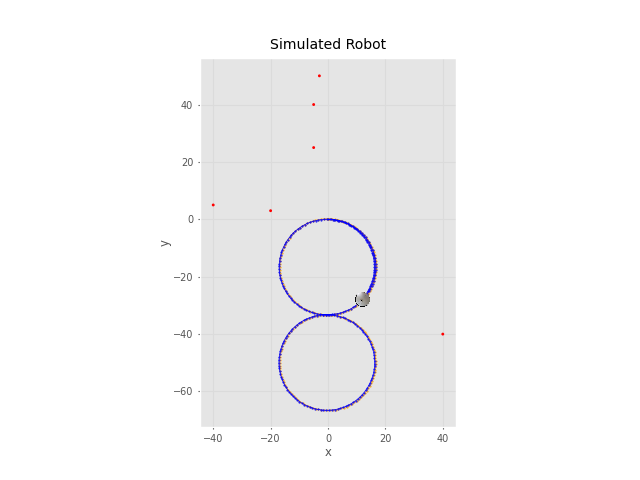
\includegraphics[width=7.0cm]{Figures/2.DeadReckoning/8_DR_noNoiseRecoder_noiseAcc.png}}
        \captionsetup{justification=centering}
        \caption{8-figure trajectory}
        \label{fig:rana}
    \end{subfigure}
\caption{No Dead-Reckoning problem}
\label{fig:map3_1}
\end{figure}

\begin{figure}[H]
    \centering
    \begin{subfigure}[b]{8.cm}
        \centering
        \frame{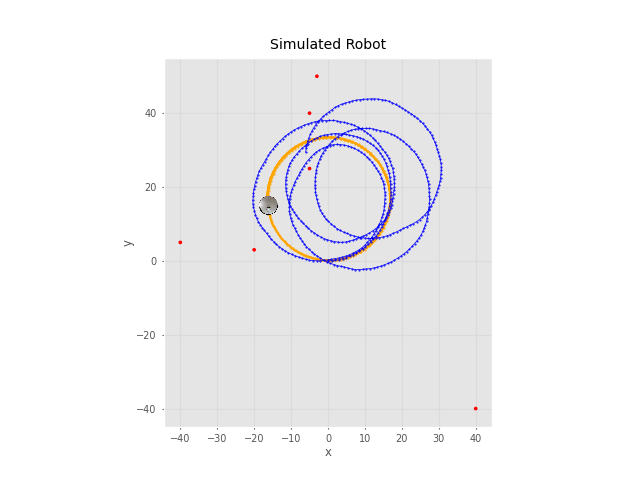
\includegraphics[width=7.00cm]{Figures/2.DeadReckoning/o_DR_mean_0.0_std_22.png}}
        \captionsetup{justification=centering}
        \caption{Circular trajectory}
        \label{fig:kermit}
    \end{subfigure}
    % \hfill
    \begin{subfigure}[b]{8.cm}
        \centering
        \frame{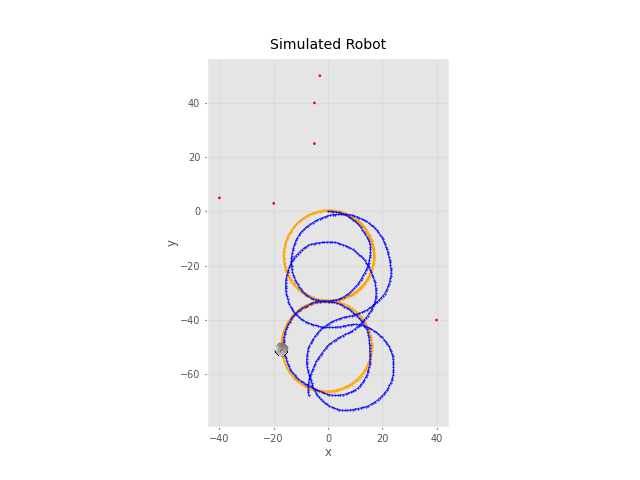
\includegraphics[width=7.0cm]{Figures/2.DeadReckoning/8_DR_mean_0.0_std_22.png}}
        \captionsetup{justification=centering}
        \caption{8-figure trajectory}
        \label{fig:rana}
    \end{subfigure}
\caption{The Dead-Reckoning problem when adding Gaussian white noise in the recorder output}
\label{fig:map3_2}
\end{figure}

\noindent
As mentioned above, the formulas which were implemented in this software were represented clearly in the \cite{Lectures}, \cite{Book} and \cite{SoftwareDesign}, so we only concentrate on issues and problems encountered during implementation. These will be discussed more in the next section.


\section{Issues}
\setcounter{figure}{0}  
During implementation, there are two issues we encountered: Encoder modeling and System modeling. These issues influence the accuracy of the localization system and the error of Dead-reckoning problem besides the noise of the sensors.
\label{sec:Issues}
\subsection{Encoder Modeling}
As mentioned above, the "ReadEncoders" function computes the measurement of this sensor from the velocity represented in the body-fixed frame of the robot ($\nu_{sk}$). Because in reality, the measurement of encoder is integer, the output of the sensor need to be rounded. This step creates error in the position of robot between the localization system and simulation even in the absence of noise on the sensor. The figure \ref{fig:map4_1}, with the output rounding, there is position error between simulation and localization system (No noise in the encoder output).

\begin{figure}[H]
    \centering
    \begin{subfigure}[b]{8.cm}
        \centering
        \frame{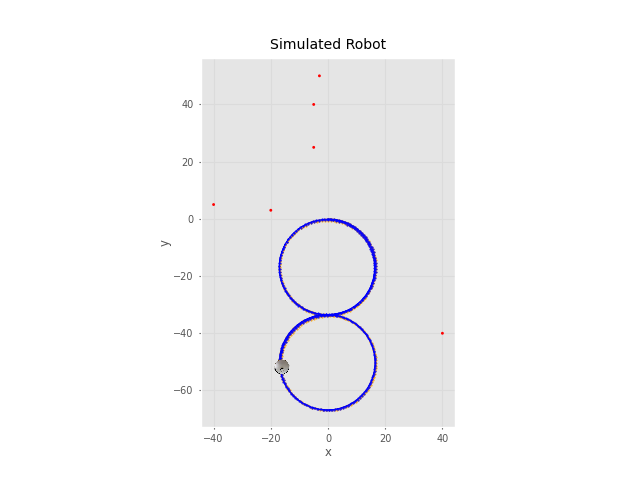
\includegraphics[width=7.00cm]{Figures/2.DeadReckoning/8_DR_Noise_noInt_1024.png}}
        \captionsetup{justification=centering}
        \caption{No rounding the output}
        \label{fig:kermit}
    \end{subfigure}
    % \hfill
    \begin{subfigure}[b]{8.cm}
        \centering
        \frame{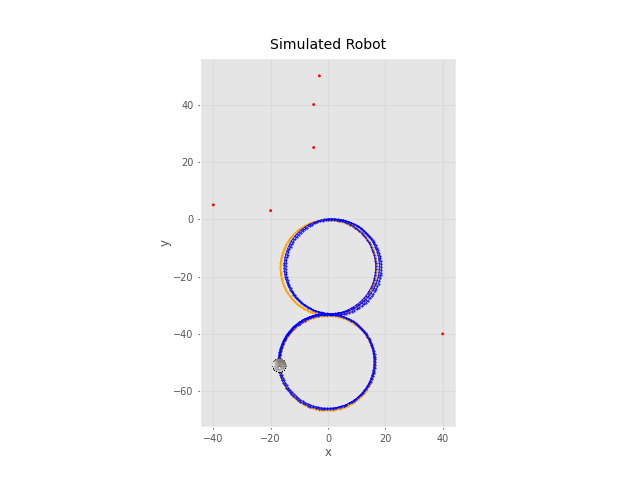
\includegraphics[width=7.0cm]{Figures/2.DeadReckoning/8_DR_Noise_int_1024.png}}
        \captionsetup{justification=centering}
        \caption{Rounding the output}
        \label{fig:rana}
    \end{subfigure}
\caption{The Dead-Reckoning comparison, number of pulses per wheel turn is 1024)}
\label{fig:map4_1}
\end{figure}

\noindent
In order to deal with this problem, solution is increasing the solution of the encoder sensor (number of pulses per wheel turn). This method helps reduce rounding error or loss of data. Because of this problem, the resolution become one of the features choosing the encoder sensor. The figure \ref{fig:map4_3} below represents the development when increasing the resolution of encoder.
\begin{figure}[H]
    \centering
    \begin{subfigure}[b]{8.cm}
        \centering
        \frame{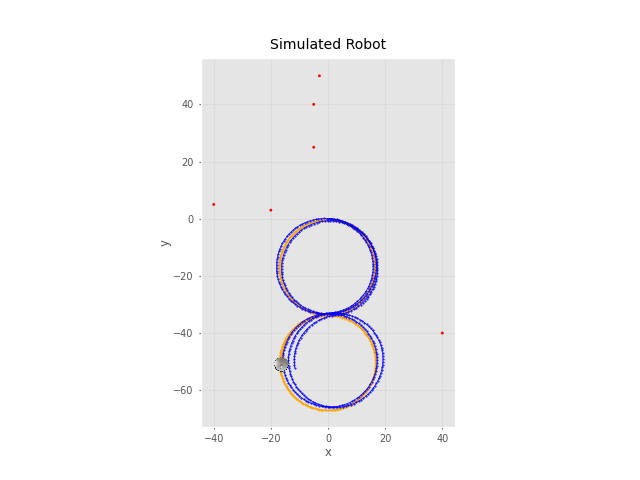
\includegraphics[width=7.00cm]{Figures/2.DeadReckoning/8_DR_Noise_int_512.png}}
        \captionsetup{justification=centering}
        \caption{number of pulses per wheel turn is 512}
        \label{fig:kermit}
    \end{subfigure}
    % \hfill
    \begin{subfigure}[b]{8.cm}
        \centering
        \frame{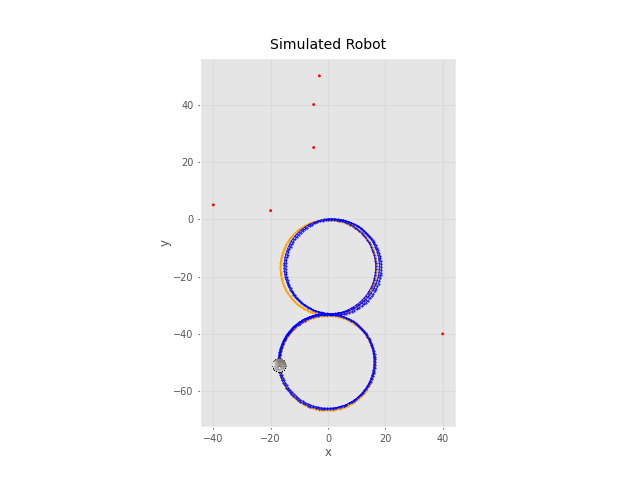
\includegraphics[width=7.0cm]{Figures/2.DeadReckoning/8_DR_Noise_int_1024.png}}
        \captionsetup{justification=centering}
        \caption{number of pulses per wheel turn is 1024}
        \label{fig:rana}
    \end{subfigure}
\label{fig:map4_2}
\end{figure}
\begin{figure}[H]
    \centering
    \begin{subfigure}[b]{8.cm}
        \centering
        \frame{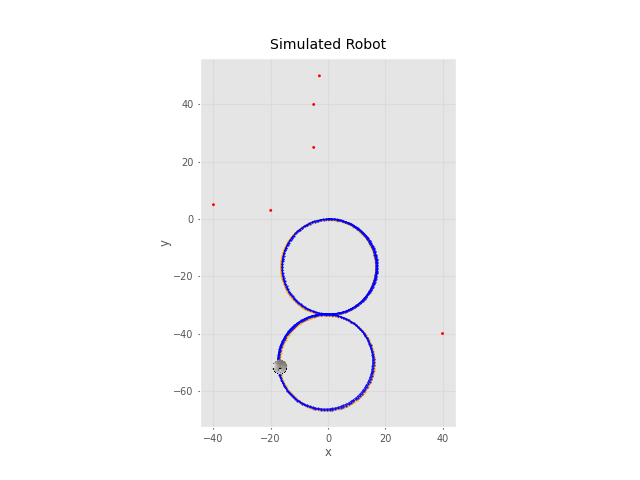
\includegraphics[width=7.00cm]{Figures/2.DeadReckoning/8_DR_Noise_int_4096.png}}
        \captionsetup{justification=centering}
        \caption{number of pulses per wheel turn is 4096}
        \label{fig:kermit}
    \end{subfigure}
    % \hfill
    \begin{subfigure}[b]{8.cm}
        \centering
        \frame{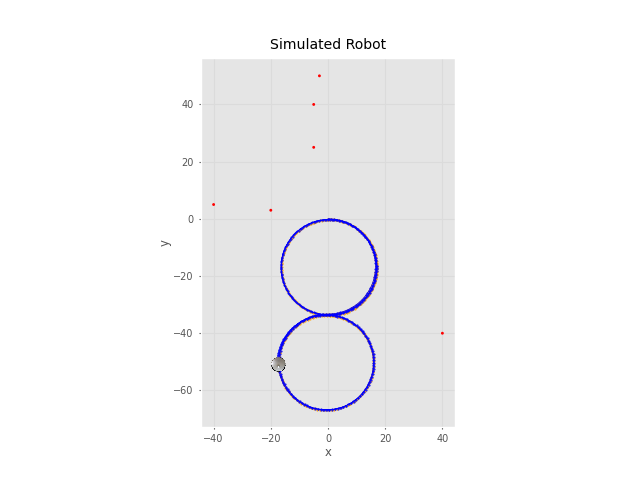
\includegraphics[width=7.0cm]{Figures/2.DeadReckoning/8_DR_Noise_int_8192.png}}
        \captionsetup{justification=centering}
        \caption{number of pulses per wheel turn is 8192}
        \label{fig:rana}
    \end{subfigure}
\caption{The development when increasing resolution of sensor}
\label{fig:map4_3}
\end{figure}
\subsection{System Modeling}
\setcounter{figure}{0}  
While in reality, the robot is a continuous system, the simulation is a discrete system running with 10Hz frequency. It bases on an assumption, where the velocity of the robot between two samples is considered being a constant and the acceleration is considered as a noise. 
\begin{equation}
\label{eq:4.1}
\eta_{sk} = \eta_{s_{k-1}} + \nu_{s_{k-1}} \Delta t
\end{equation}
However, This assumption is not true. It is one of causes leading to Dead-Reckoning problem of the robot. And this is the cumulative error over time which is increasing gradually when simulation period rises. 

\noindent
The solution for this situation is increase the frequency of the simulation. So how much increase is enough? It depends on the acceleration or changing speed of robot velocity. The increase need to satisfy the above assumption. 

\section{Conclusions}
\label{sec:Conclussions}
In conclusion, through the lab, we have an overview of a robot simulation system including simulation components and localization components. More specifically, with the simulation block, we need to model the robot and its sensors, while the localization block requires computing the robot's state from the sensor's measurement signals. With the localization system being used, there is a Dead-reckoning problem when noise is added to the encoder sensor's measurement signal. Besides, the Dead-reckoning problemproblem is also the result of encoder sensor modeling and robot system modeling.

%++++++++++++++++++++++++++++++++++++++++
% References section will be created automatically 
% with inclusion of "thebibliography" environment
% as it shown below. See text starting with line
% \begin{thebibliography}{99}
% Note: with this approach it is YOUR responsibility to put them in order
% of appearance.



\begin{thebibliography}{99}
\bibitem{Lectures}
Pere Ridao. "MR1-23-24-Introduction". Version 0.1. October 02, 2023

\bibitem{Book}
Pere Ridao. "Probabilistic Robot Localization and Mapping". Version 2.0. September, 2022

\bibitem{SoftwareDesign}
Pere Ridao. "prpy: Probabilistic Robot Localization Python Library". Version 0.1. October 02, 2023

\end{thebibliography}

\end{document}